\begin{figure}[H]
\centering
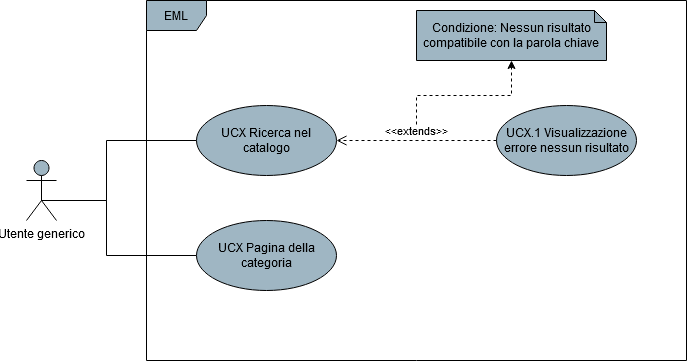
\includegraphics[scale=0.6]{res/UseCase/Immagini/NavigazioneCatalogoGenerale}
\caption{Diagramma UML per modulo di navigazione del catalogo}
\end{figure}
\subsubsection{UC9 - Ricerca nel catalogo digitale}
\begin{itemize}
\item \textbf{Attori primari}: utente generico;
\item \textbf{Descrizione}: l'utente può effettuare una ricerca tra tutti i prodotti in vendita nella piattaforma attraverso la digitazione di una parola o frase chiave nella barra di ricerca;
\item \textbf{Scenario Principale}: l'utente seleziona la barra di ricerca, inserisce la parola chiave corrispondente al prodotto desiderato e infine visualizza una lista di prodotti compatibili con la parola digitata;
\item \textbf{Estensioni}:
\begin{itemize}
\item se non viene trovato nessun risultato compatibile con la parola chiave viene visualizzato un messaggio di errore [\textbf{UC10}];
\end{itemize}
\item \textbf{Precondizione}: l'utente si trova sulla piattaforma e necessita di fare una ricerca per trovare un prodotto specifico;
\item \textbf{Postcondizione}: la ricerca è avvenuta e restituisce come risultato l'insieme di prodotti compatibili con la parola chiave digitata.
\end{itemize}
\subsubsection{UC10 - Visualizzazione errore nessun risultato ricerca}
\begin{itemize}
\item \textbf{Attori primari}: utente generico;
\item \textbf{Descrizione}: l'utente visualizza un messaggio di errore che lo informa che la ricerca effettuata sulla parola chiave da lui inserita non ha prodotto nessun risultato.
\item \textbf{Scenario Principale}: l'utente effettua una ricerca sul catalogo digitale con una parola chiave che non ha riferimenti a nessun prodotto;
\item \textbf{Precondizione}: l'utente si trova sulla piattaforma ed ha effettuato una ricerca;
\item \textbf{Postcondizione}: viene visualizzato un messaggio che informa l'utente di non aver trovato risultati compatibili con quanto digitato nella barra di ricerca.
\end{itemize}
\subsubsection{UC11 - Visualizzazione pagina della categoria}
\begin{itemize}
\item \textbf{Attori primari}: utente generico;
\item \textbf{Descrizione}: l'utente può accedere ad una pagina contenente un insieme di prodotti listati facenti parte di una specifica categoria. In questa pagina, chiamata anche PLP\ped{G}, l'utente ha a disposizione ulteriori strumenti per visualizzare e selezionare per l'acquisto i prodotti da lui desiderati.
\item \textbf{Scenario Principale}: l'utente clicca sulla categoria di prodotti da lui desiderata;
\item \textbf{Precondizione}: l'utente si trova sulla piattaforma e necessita di visualizzare tutti i prodotti contenuti in una specifica categoria;
\item \textbf{Postcondizione}: l'utente accede alla PLP\ped{G} corrispondente alla categoria desiderata.
\end{itemize}
\begin{figure}[H]
\centering
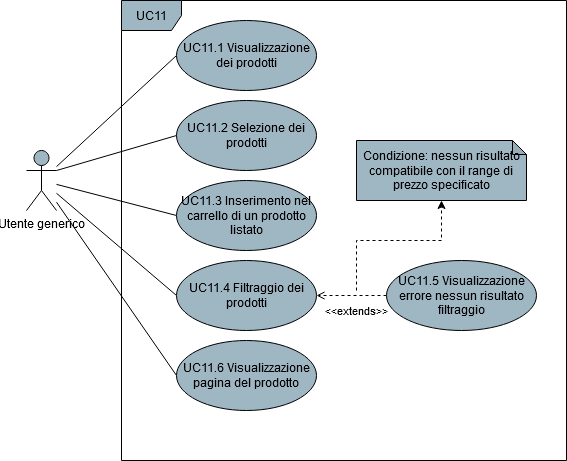
\includegraphics[scale=0.6]{res/UseCase/Immagini/VisualizzazionePaginaCategoria}
\caption{Diagramma UML per UC11 - Visualizzazione pagina della categoria}
\end{figure}